\documentclass{article}

\usepackage{graphicx}
\usepackage{hyperref}
\usepackage{tabularx}
\usepackage{amsmath}
\usepackage{amssymb}
\usepackage{boxedminipage2e}

\title{Project: Movie Recommendation Engine}
\author{Karsten Poddig}

\begin{document}

\maketitle

\begin{abstract}
The project described in this report is a Movie Recommendation Engine\\[2ex]
\textbf{Github Repo:}\\
\url{https://github.com/KarstenPoddig/django_movie_project}\\[2ex]
\textbf{Keywords:} Data Science, Data Engineering, Statistical Dashboard, Analytics, Movie Recommendation Engine, kNN-Regression, Hierarchical Clustering,  Python, Django, Docker, Kubernetes, Continious Integration, Continious Development, Google Cloud Platform, SQL, PostgreSQL, JavaScript, Git, GitHub


\includegraphics[scale=0.055]{logos/python_logo.png}
\hspace{5mm}

\includegraphics[scale=0.1]{logos/scikit_learn_logo.png}
\hspace{5mm}

\includegraphics[scale=0.04]{logos/django_logo.png}
\hspace{5mm}

\includegraphics[scale=0.035]{logos/postgresql_logo.png}
\hspace{5mm}

\includegraphics[scale=0.12]{logos/docker_logo.png}
\hspace{5mm}

\includegraphics[scale=0.08]{logos/kubernetes_logo.png}
\hspace{5mm}

\includegraphics[scale=0.015]{logos/gcp_logo.png}
\hspace{5mm}

\includegraphics[scale=0.15]{logos/js_logo.png}
\hspace{5mm}
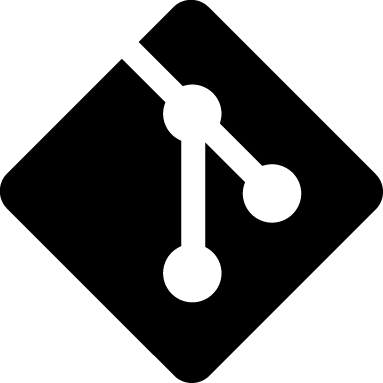
\includegraphics[scale=0.05]{logos/git_logo.png}
\hspace{5mm}

\includegraphics[scale=0.04]{logos/github_logo.png}

\end{abstract}

\tableofcontents

\newpage


% #################### Introduction #######################################
\section{Introduction}






% #################### Usage of App #######################################
\section{App functionalities}

This section provides a quick overview of the functionalities of this app. The following functionalities can be accessed without an account:

\begin{itemize}
	\item Search Movies
	\item Search for similar movies for a specific movie
\end{itemize}
The main functionalities require an account. These functionalities include

\begin{itemize}
	\item Rate Movies
	\item Get Suggestions based on your ratings
\end{itemize}
Since the main purpose of this project is to provide movie suggestions I recommend to sign in if you want to explore this app. You can do this by creating an account and create your own ratings. But rating a sufficient number of movies can be time consuming, so if you want to go on fast and simply want to explore what how this app works you can simply use the following account with exisiting ratings:\\

\begin{tabular}{|l|l|}
\hline
username & testuser \\
\hline password & password\\
\hline
\end{tabular}\\

The following subsections guide you through the app. But since the app should be somehow intuitive you can also skip these subsections.

\subsection{Sign up / Sign In}

\subsubsection*{Sign Up}

Click on the button in the right top corner and enter all necessary data.\\[2ex]
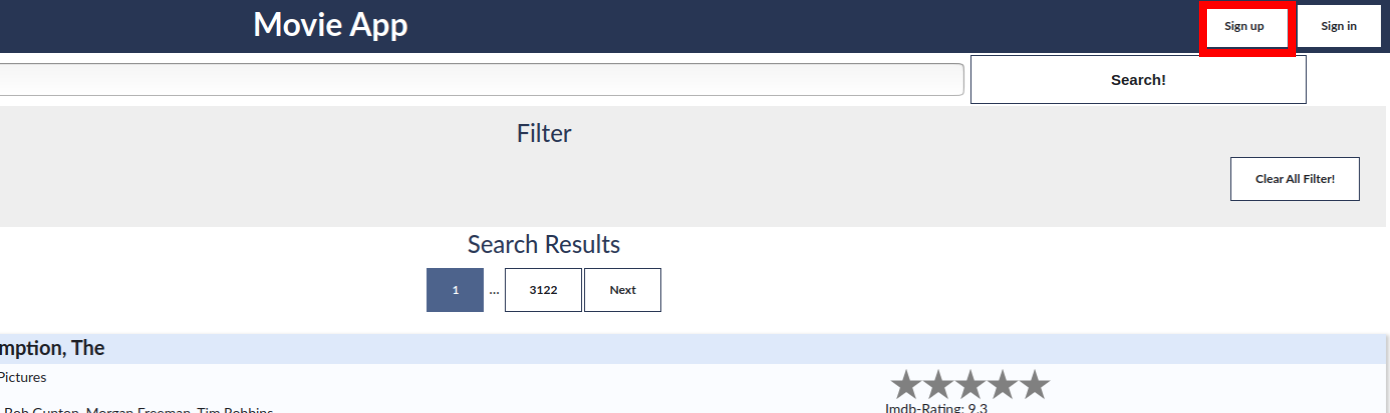
\includegraphics[scale=0.3]{screenshots_app/sign_up.png}\\

\subsubsection{Sign In}

Click on the button in the right top corner and all necessary data.\\[2ex]
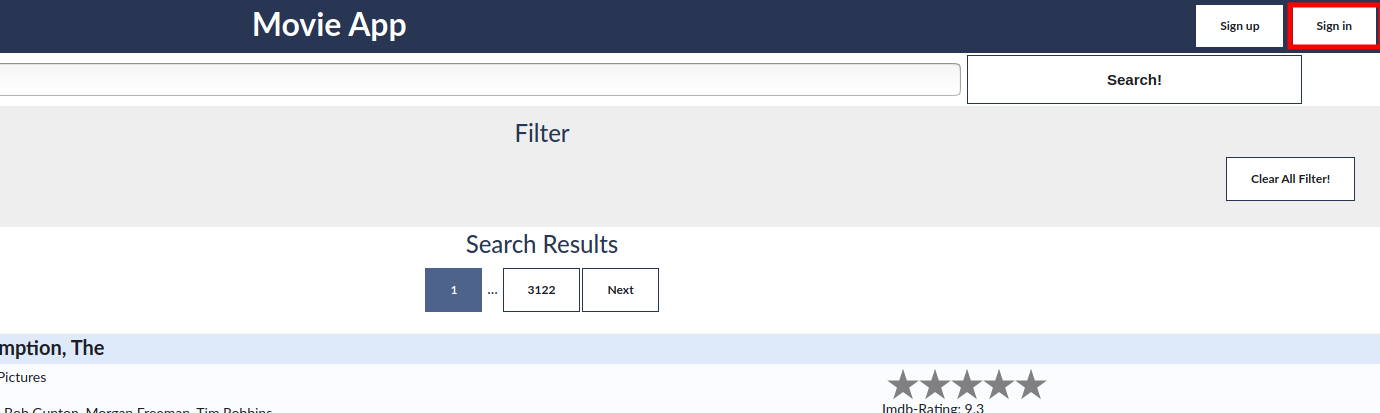
\includegraphics[scale=0.3]{screenshots_app/sign_in.png}\\
Also you are redirected to the Sign In - page if you are accessing areas which require a login (like Rated Movies, etc.)


\subsection{Search Movies}

Click on the link 'All Movies' in the left bar. You will see a list of all movies in the database with the regarding details.
To search a movie you can enter parts of title (green area) and optionally set certain filter critria (yellow area). The results are ordered decreasingly by popularity (total number of ratings).\\[2ex]
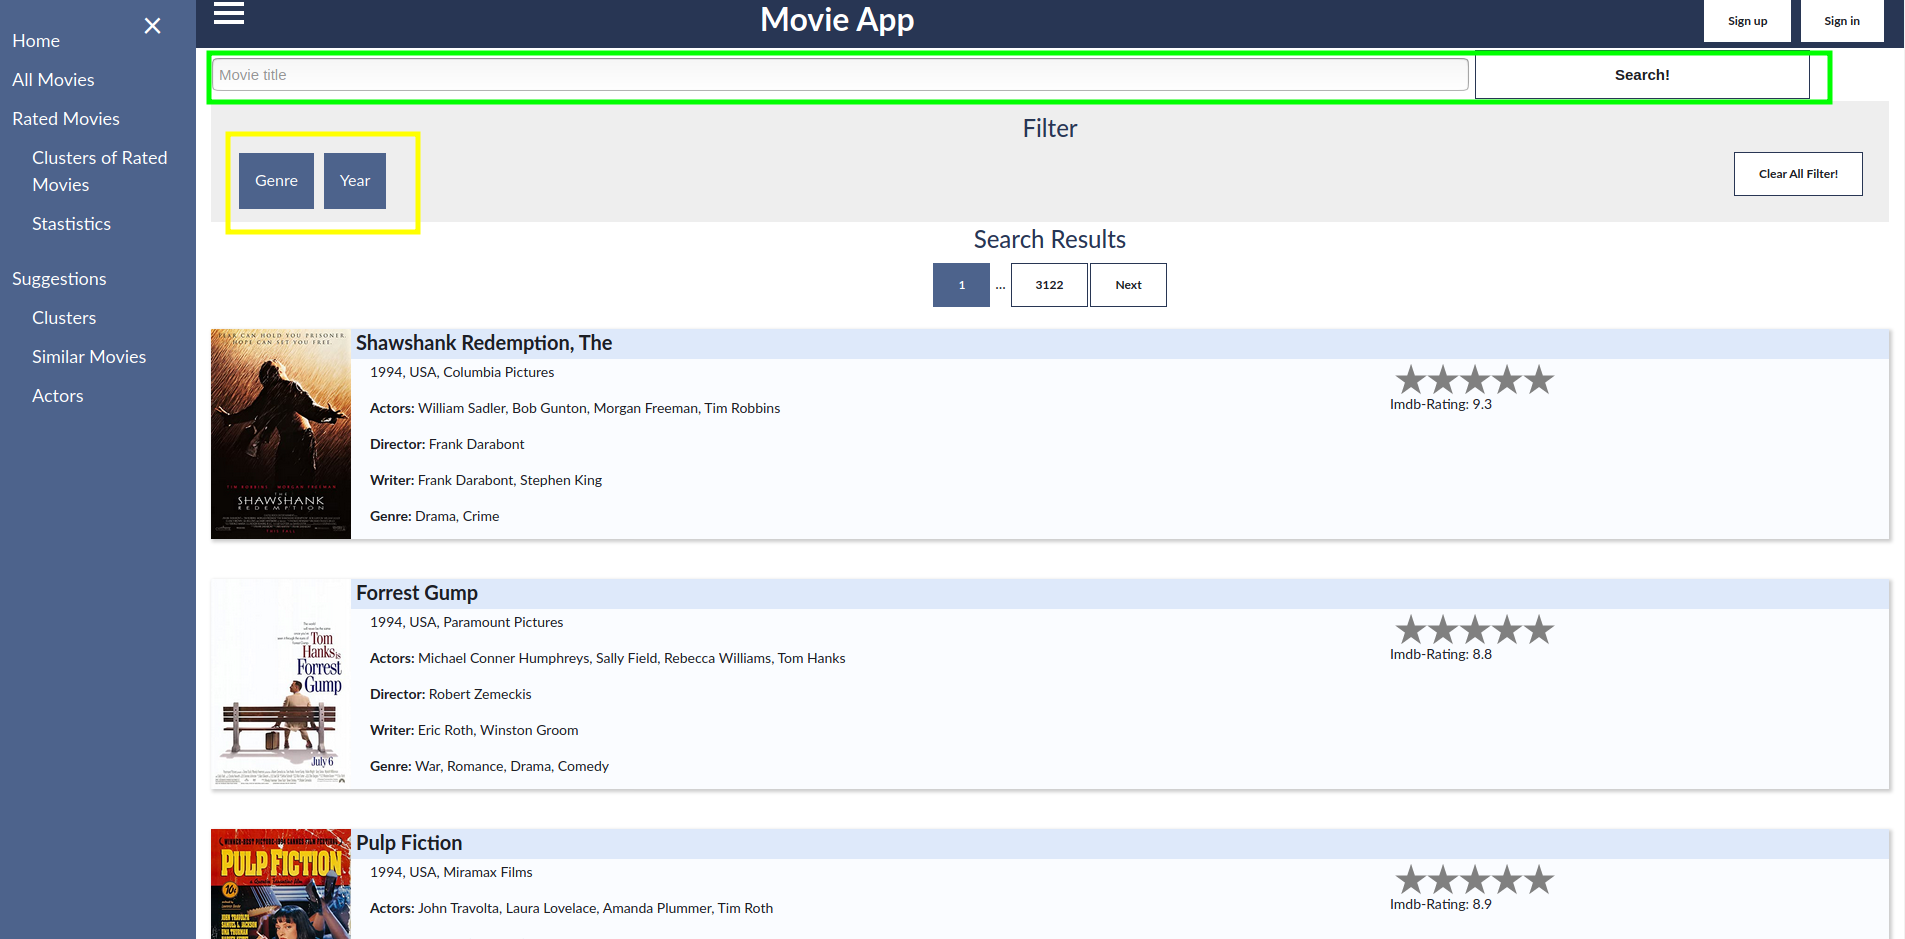
\includegraphics[scale=0.25]{screenshots_app/all_movies.png}\\

For example a search for movies with the term 'Bad' in the title with the Genre Action in the 2000s will look like the following:\\[2ex]
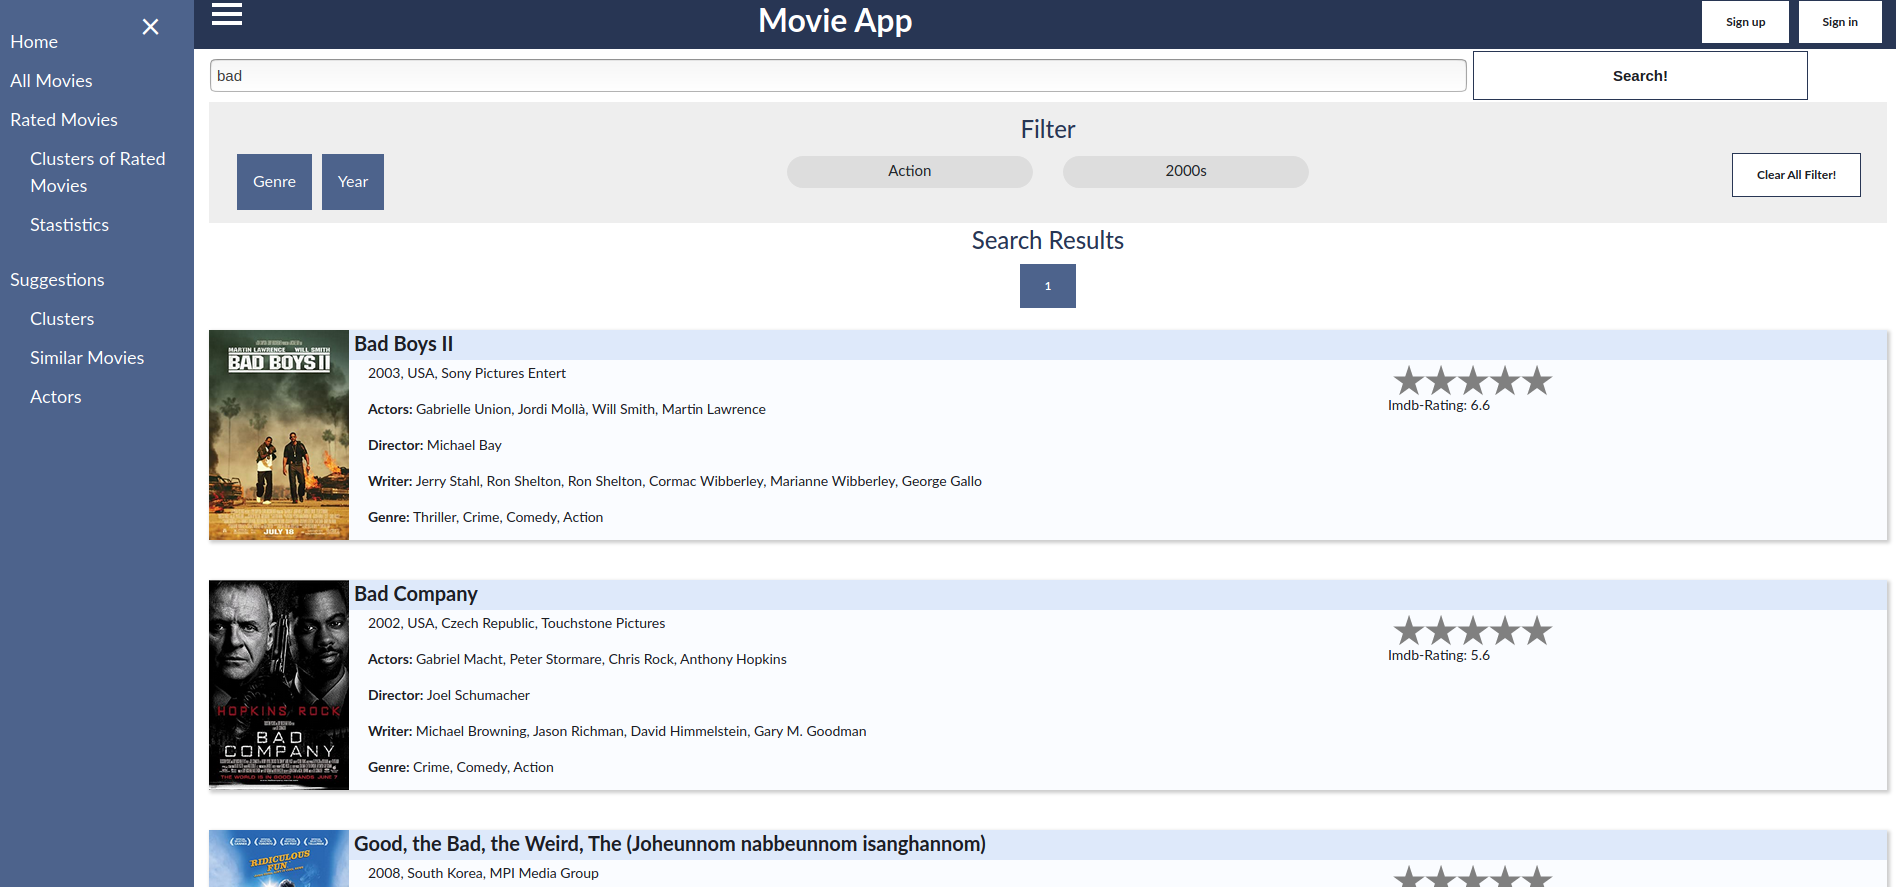
\includegraphics[scale=0.2]{screenshots_app/all_movies_ex1.png}\\


\subsection{Rate Movies}

Once you are logged in you can rate movies. Just enter the page 'All Movies', search the movie you want to rate and click on the regarding rating (red area in the following picture). If you choose a rating of 0 stars an existing rating will be deleted.\\[2ex]
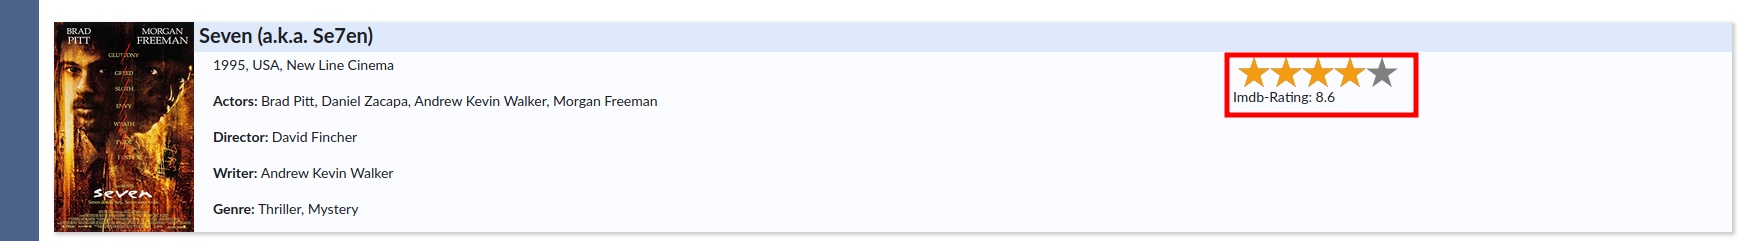
\includegraphics[scale=0.3]{screenshots_app/rate_movie_ex1.png}\\


\subsection{View Rated Movies}

At some point you maybe want to take a look at the movies you already rated. The links for the sections 2.4.1-2.4.3 are displayed in the following picture.
\\[2ex]
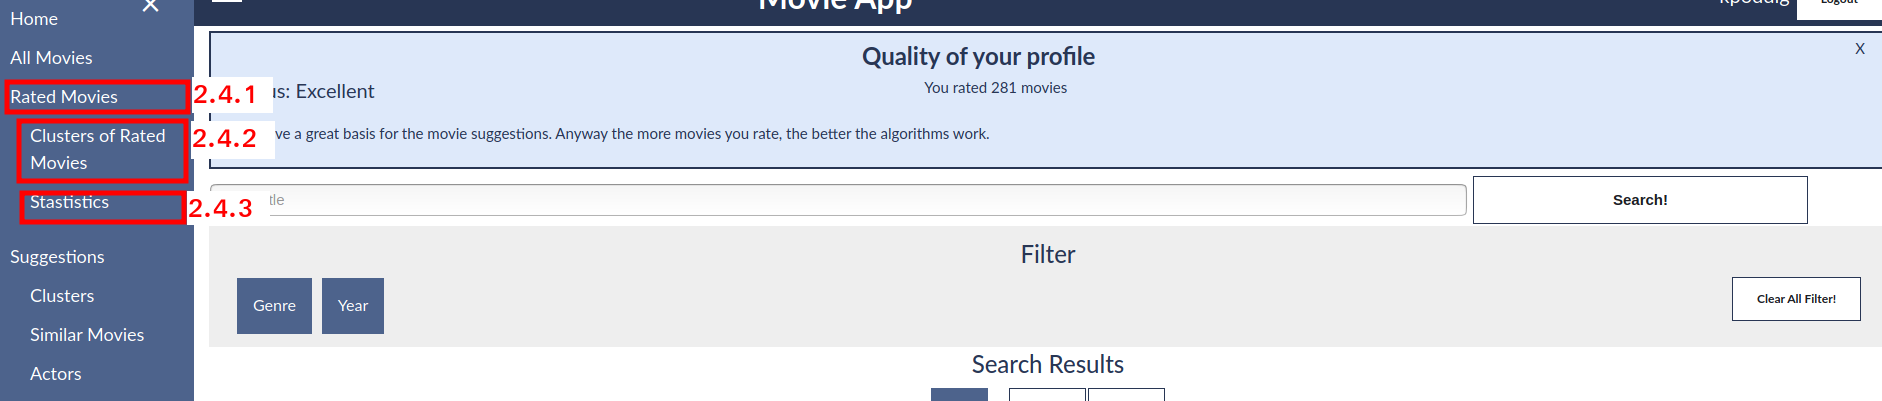
\includegraphics[scale=0.3]{screenshots_app/rated_movies_navigation.png}\\


\subsubsection{Movies with Details}

This is basically the same page as 'All Movies' (section 2.2) with the exception that just rated movies are listed here. You can search and navigate through your rated movies in the same way as in section 2.2.

\subsubsection{Clustered Movies}

To determine better suggestions your rated movies are clustered. Take a look at section. Basically each cluster (each line) contains movies which are similar to each other. Factors which imply a similarity could be the genre, the production year, the atmosphere, actors, etc. For a better understanding what similarity in this context means I again refer to Section .... .
If you want to update the clustering hit the button 'Refresh Cluster' (marked red).\\[2ex]
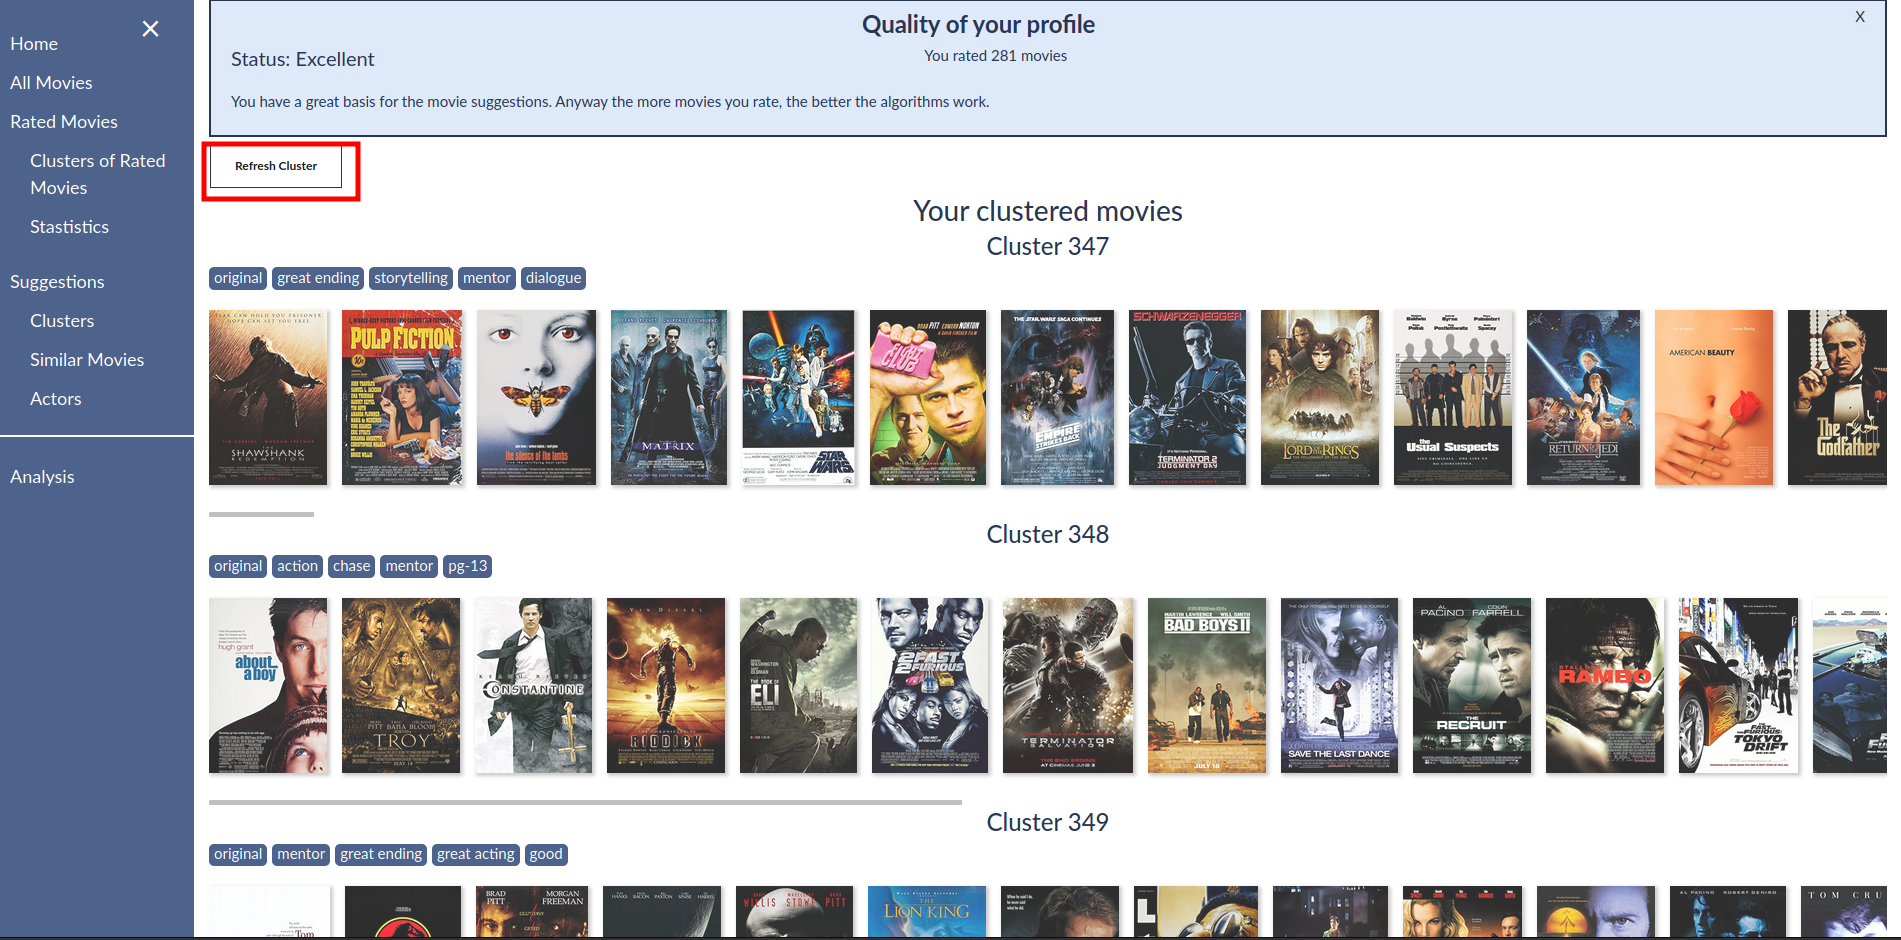
\includegraphics[scale=0.3]{screenshots_app/rated_movies_clustered.png}\\


\subsubsection{Statistics}

This page provides a statistical dashboard for your ratings.\\[2ex]
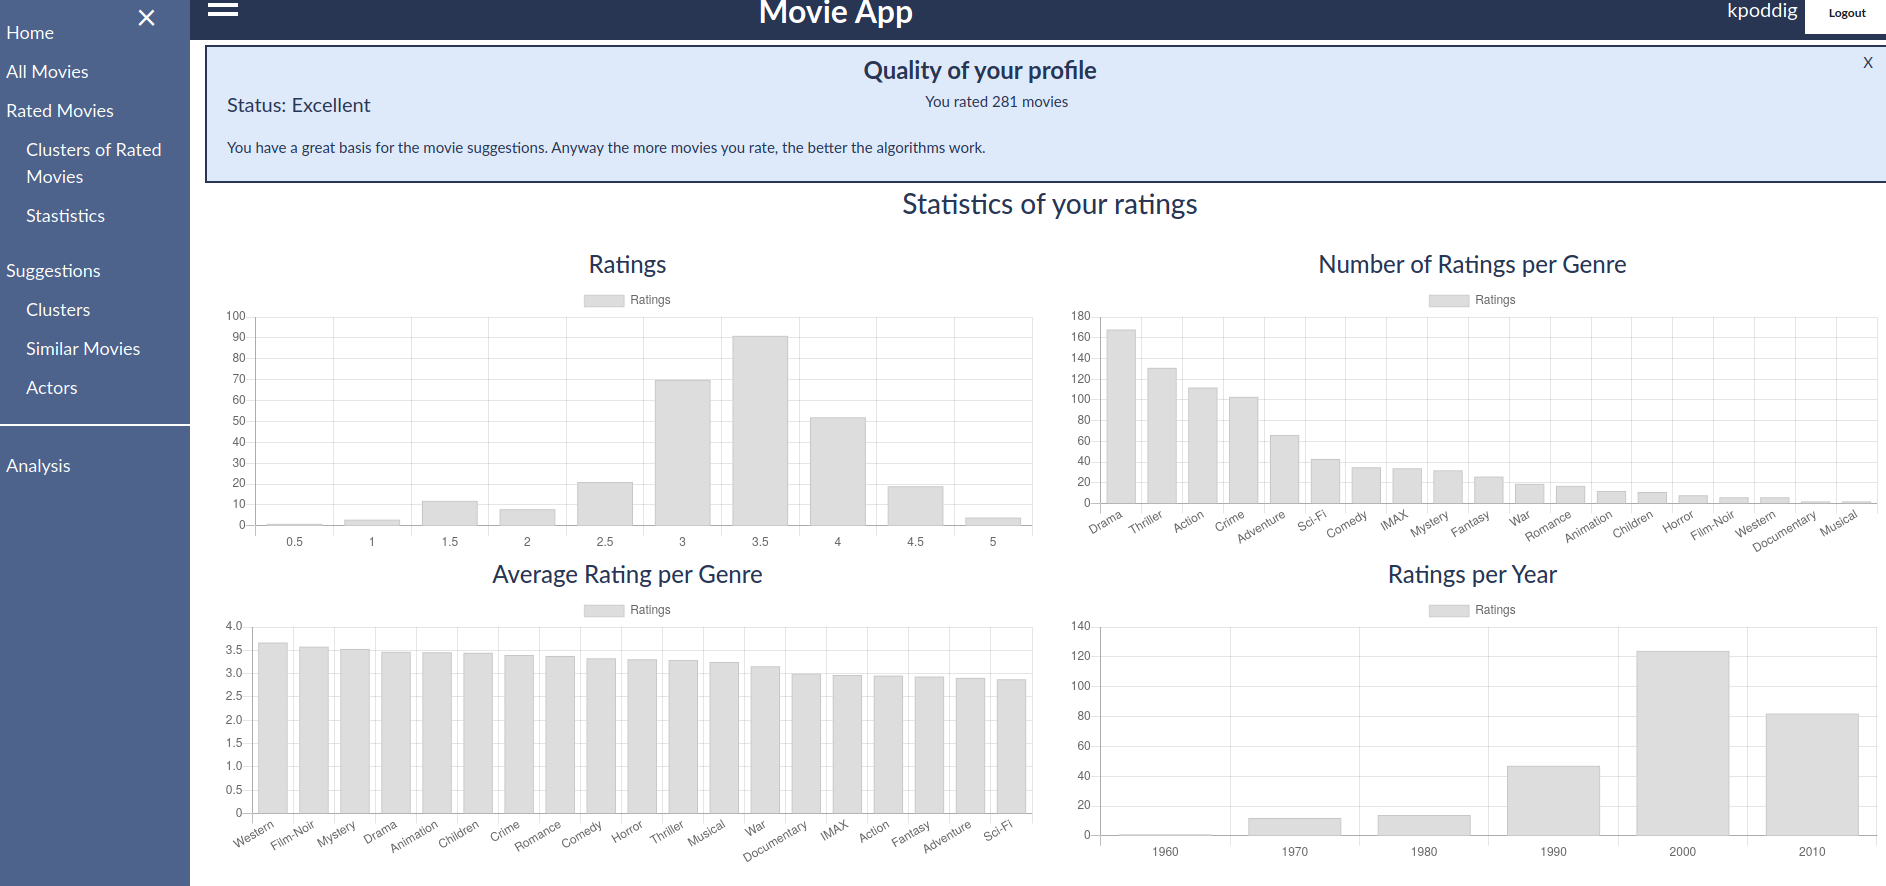
\includegraphics[scale=0.2]{screenshots_app/rated_movies_statistics.png}\\





\subsection{View Suggestions}

Now it comes to the core functionality of the app. The following picture displays the links to the sections 2.5.1 - 2.5.3.

\subsubsection{Suggestions based on clusters}



\subsubsection{Search Similar Movies}



\subsubsection{Suggestions based on Actors}





% #################### Data Science Part #################################
\section{Data Science Part}

In this section the algorithm on which the movie recommendation engine are explained.

\subsection{Notation}

Let $U = \{ u_i \}_{1 \leq i \leq m}$ be the set of all users. The set of all movies is denoted with $M = \{ m_j \}_{1 \leq j \leq n}$. The set $R$ contains all tuples of users and movies for which a rating exists, i.e.
\[ R = \left\{ (u, m)~|~\textrm{if user }u\textrm{ rated movie }m\right\}\subseteq U\times M.\]
If user $u$ rates the movie $m$ (and therefore $(u,m)\in R$)  the rating is denoted by $r_{u_i, m_j}$. The set off all ratings is then $\{ r_{u, m}\}_{(u,m)\in R}$.

\begin{eqnarray}
r &:& R \rightarrow \{0.5, 1, 1.5, 2, 2.5, 3, 3.5, 4, 4.5, 5\}\nonumber
\end{eqnarray}


\subsection{Similarity and Distance}

The most important part to determine movie suggestions is the concept of similarity of movies. As a similarity measure we use the cosine similarity.\\[2ex]
\begin{boxedminipage}{\textwidth}
\textbf{Short Excourse: Cosine Similarity}\\[2ex]
Let $x, y \in \mathbb{R}^n$. Then the cosine similarity of these vectors is defined as
\[ similarity(x,y) := \frac{\langle x,y\rangle}{\lVert x\rVert \lVert y \rVert} = \frac{\sum_{i=1}^n x_i y_i}{\sqrt{\sum_{i=1}^nx_i^2}\sqrt{\sum_{i=1}^nx_i^2}},\]
where $\langle x,y\rangle$ is the scalar product (or inner product) of the two vectors and $\lVert x \rVert$ is the euclidian norm (l2 norm) of the vector $x$.
The cosine similarity is in general a value between -1 and  1. The highest similarity is 1 and is achieved if and only if $x$ and $y$ there is a $\lambda > 0$ such that $y = \lambda x$.
\end{boxedminipage}\\[2ex]
We will apply the concept of the cosine similarity in the following way. Let $m, m' \in M$ be two arbitrary movies. The vector for each movie is the vector of ratings. If a user didn't rate a movie then the value in the vector is defined as zero. Written technically that means
\[ \bar{r}_m = \begin{pmatrix} \bar{r}_{u_1,m} \\ .. \\ \bar{r}_{u_m, m}\end{pmatrix},~\text{where }\bar{r}_{u_i, m} := \begin{cases} r_{u_i,m}~\text{if }(u_i,m)\in R \\ 0~\text{else}\end{cases}.\]
So now we get our similarity of movie $m, m'$ as
\[ similarity(m,m'):= \frac{\langle \bar{r}_{m}, \bar{r}_{m'}\rangle}{\lVert \bar{r}_m \rVert \lVert \bar{r}_{m'} \rVert }.\]
Notice: Since all values in the vectors which appear here are greater or equal zero the similarity measure is always between zero and one. This makes the ongoing computations more comfortable, since we don't have to deal with negative similarites.
The more parallel the vectors $\bar{r}_m, \bar{r}_{m'}$ are, the higher the  is the similarity of the movies $m$ and $m'$.\\
Speaking freely: If two movies in general are rated similar by the same users then the movies are considered as similar.\\
\textbf{Example:} In section 2.5.2 it is shown that we can search the most similar movies 




\subsection{Prediction of Rating}

Now it comes to the prediction of ratings: Let's say there is a user $u\in U$ and some movie $m\in M$ which is not already rated by $u$, that means $m\notin M_u$ (as defined in section 3.1. $M_u$ is the set of all movies which $u$ did already rate).\\
The prediction $\hat{r}_{u,m}$ is simply the average value of the rating $(r_{u,m})_{m\in M}$ weighted by similarity. Of course the intuition of this approach is more similar movies to $m$ should have a higher impact on the prediction.\\
Furthermore there are at most the 15 movies included. Using just a low number of movies for the prediction yields better results than using all movies. The number $k=15$ is chosen because heuristically for this value the evaluation metrics has shown the smallest error for the predictions (see subsection 3.6).\\
This algorithm is known as the $k$ Nearest Neighbour Regression (with $k=15$).\\[2ex]
Expressed in a more technical way: Let $u\in U$, $m\notin M_u$. Then
\[ \hat{r}_{u,m} := \sum_{i=1}^{\min(15, |M_u|)} \left(\frac{similarity(m^{(i)}, m)}{\sum_{i=1}^{\min(15, |M_u|} similarity(m^{(i)}, m)} \right)~r_{u, m^{(i)}},\]
where $(m^{(1)}, m^{(2)}, ....)\in M_u$ are the movies rated by $u$ sorted by the similarity to $m$. That means $(similarity(m^{i},m))_i$ is decreasing.


\subsection{Clustering of Rated movies for a user}

The next step is the clustering of rated movies. What is the purpose for this step? At first one could think to simply compute the rating predictions for all movies and then suggest the movies with the highest predicted values to the user. But in reality often people like different kind of movies. Depending on your mood, etc. you maybe want to watch a movie of a certain genre, topic, athmosphere and so on. Therefore the rated movies will be clustered and then for each cluster suggestions will be determined.\\
The clustering algorithm to compute these clusters is the AgglomerativeClustering provided by the package scikit-learn. This algorithm needs the information which distance should be used to cluster the objects. Here we will use the option 'precomputed' and provide a matrix which is based on the similarity matrix in section 3.2 $(similarity(m,m'))_{m,m'\in M}$. The number of clusters also needs to be set at the beginning.\\[2ex]
\begin{boxedminipage}{\textwidth}
\textbf{Creation of distance matrix}\\[2ex]
The distance between the objects is often simply defined as the inverse of the similarity. But in this case there is a problem with this approach:\\
Let's take two movies. First we take $m_1$ is 'Harry Potter and the Goblet of Fire'. The second movie $m_2$ is 'Burn After Reading'. Then we enter these movies in the similarity view (section 2.5.2) and check the result:\\
As you can see the similarities for $m_1$ are much higher then for $m_2$. Anyway the similarity search works good for both movies. This is an example for the following relation: The similarities for popular movies are in general much higher then for less popular movies. If one would simply take the inverse of the similarity as the distance the result is one big cluster including all blockbuster and some very small cluster with relatively unpopular movies.\\
Therefore here we take the following approach: Instead of focusing on the absolute similarity values the distance is determined by the position in the similarity list. That means to compute the 
\end{boxedminipage}\\[2ex]



\section{Final Predictions}


\subsection{Evaluation of Prediction Algorithm}


\subsection{Discussion}


% #################### Data Engineering Part #############################
\section{Data Engineering Part}

\subsection{Source of Data}

MovieLen, Imdb-API
Own ratings


\subsection{Google Cloud SQL}






\end{document}